\documentclass[12pt, a4paper]{report}
\special{papersize=210mm, 297mm}
\usepackage[english]{babel}
\usepackage[utf8]{inputenc}
\usepackage[left=2.5cm, right=2.5cm, top=2.5cm]{geometry}
\renewcommand{\baselinestretch}{1.4}
\usepackage[toc,page]{appendix}

\usepackage{amsmath}
\usepackage{graphicx}
\usepackage{float}
\graphicspath{{images/} {diagrams/}}

%\usepackage{showframe}
\usepackage{fullpage}

\usepackage{url}
%\usepackage{natbib} % for author-date citation \citep{}, \citet[]
%\usepackage{hyperref}
%\usepackage[nottoc]{tocbibind}
\usepackage{listings}
\usepackage{verbatim}
\usepackage{color}

\usepackage{biblatex}

\definecolor{dkgreen}{rgb}{0,0.6,0}
\definecolor{gray}{rgb}{0.5,0.5,0.5}
\definecolor{mauve}{rgb}{0.58,0,0.82}

\lstset{frame=tb,
	 language=java,
	aboveskip=5mm, belowskip=3mm, showstringspaces=false,
	columns=flexible, basicstyle={\small\ttfamily},
	numbers=none, numberstyle=\tiny\color{gray},
	keywordstyle=\color{blue},
	commentstyle=\color{dkgreen},
	stringstyle=\color{mauve},
	breaklines=true,
	breakatwhitespace=true,
	tabsize=3
}


\usepackage{multirow}
\usepackage{array}
\newcolumntype{L}[1]{> {\raggedright\let\newline\\\arraybackslash\hspace{0pt}}m{#1}}
\newcolumntype{C}[1]{>{\centering\let\newline\\\arraybackslash\hspace{0pt}}m{#1}}
\newcolumntype{R}[1]{>{\raggedleft\let\newline\\\arraybackslash\hspace{0pt}}m{#1}}

\pagenumbering{roman}

\begin{document}

%======================================================================

\begin{titlepage}

\newcommand{\HRule}{\rule{\linewidth}{0.5mm}} % Defines a new command for the horizontal lines, change thickness here

\center % Center everything on the page

%----------------------------------------------------------------------------------------
%	LOGO SECTION
%----------------------------------------------------------------------------------------

\vspace{-20pt}

\includegraphics[width=100pt]{FMI-03.png}\\[1.0cm] % Include a department/university logo - this will require the graphicx package
 
\textsc{\LARGE West University of  Timisoara}\\[0.5cm] % Name of your university/college
\textsc{\Large Faculty of Mathematics and Computer Science}\\[0.5cm] % Major heading such as course name
\textsc{\large Study Program: \\Computer Science in English}\\[3cm] % Minor heading such as course title

%----------------------------------------------------------------------------------------
%	TITLE SECTION
%----------------------------------------------------------------------------------------

\textsc{\Huge Bachelor Thesis}\\[5cm]

%\HRule \\[0.5cm]
%{\huge \bfseries Simplified Transport Layer Security}
%\\[0.4cm]
%{\huge \bf implementation}\\[3cm] % Title of your document
%\HRule \\[1.5cm]
 
%----------------------------------------------------------------------------------------
%	AUTHOR SECTION
%----------------------------------------------------------------------------------------

%\textsc{\huge Intermediate Report}

\begin{minipage}{0.4\textwidth}
\begin{flushleft} \large
\textbf{COORDINATOR:}\\
Conf. Dr. Marc Eduard \textsc{Fr\^incu} % Coordinator
\end{flushleft}
\end{minipage}
~
\begin{minipage}{0.4\textwidth}
\begin{flushright} \large
\textbf{GRADUATE:} \\
Bulz \textsc{Gabriel} % Student's Name
\end{flushright}
\end{minipage}\\[1cm]


%----------------------------------------------------------------------------------------
%	DATE SECTION
%----------------------------------------------------------------------------------------
\vfill
{\large Timi\c{s}oara \\2018}\\ % Date, change the \today to a set date if you want to be precise

 
%----------------------------------------------------------------------------------------

%\vfill % Fill the rest of the page with whitespace

\end{titlepage}

% =====================================================================

% second title page. as requested by UVT

\begin{titlepage}

\newcommand{\HRule}{\rule{\linewidth}{0.5mm}} % Defines a new command for the horizontal lines, change thickness here

\center % Center everything on the page

%----------------------------------------------------------------------------------------
%	LOGO SECTION
%----------------------------------------------------------------------------------------

\vspace{3cm}
%
\includegraphics[width=100pt]{FMI-03.png}\\[1.0cm] % Include a department/university logo - this will require the graphicx package


\textsc{\LARGE West University of  Timisoara}\\[0.5cm] % Name of your university/college
\textsc{\Large Faculty of Mathematics and Computer Science}\\[0.5cm] % Major heading such as course name
\textsc{\large Study Program: \\Computer Science in English}\\[6cm] % Minor heading such as course title


%----------------------------------------------------------------------------------------
%	TITLE SECTION
%----------------------------------------------------------------------------------------

%\textsc{\Huge Master Dissertation}\\[2cm]

%\HRule \\[0.5cm]
{\Huge \bfseries Prezicerea zonelor inundabile}
\\[0.4cm]
{\Huge \bf folosind imagini satelitare}\\[5cm] % Title of your document
%\HRule \\[1.5cm]
 
%----------------------------------------------------------------------------------------
%	AUTHOR SECTION
%----------------------------------------------------------------------------------------

%\textsc{\huge Intermediate Report}

\begin{minipage}{0.4\textwidth}
\begin{flushleft} \large
\textbf{COORDINATOR:}\\
Conf. Dr. Marc Eduard \textsc{Fr\^incu} % Coordinator
\end{flushleft}
\end{minipage}
~
\begin{minipage}{0.4\textwidth}
\begin{flushright} \large
\textbf{GRADUATE:} \\
Bulz \textsc{Gabriel} % Student's Name
\end{flushright}
\end{minipage}\\[1cm]

%----------------------------------------------------------------------------------------
%	DATE SECTION
%----------------------------------------------------------------------------------------
\vfill
{\large Timi\c{s}oara\\ 2018}\\ % Date, change the \today to a set date if you want to be precise

 
%----------------------------------------------------------------------------------------

%\vfill % Fill the rest of the page with whitespace

\end{titlepage}

\begin{abstract} %begin abstract  
%The abstract should have one page and should be a compact presentation of the dissertation.
\vspace{1.0cm}



Floods are without doubt the most devastating natural disasters, striking numerous regions in the world each year. During the last decades due the increased frequency of heavy rain and a continuously increasing concentration of population near water regions a lot of assets and lives were lost.

That is the reason why a system that can create a flood forecasting is  

To process the resulted images we will use a library in python called GDAL which can handle that specific type of files (.tif)

In the first part we will try to identify the areas nearby the rivers and lakes (because that areas are more likely to be flooded), and in the second part we will try to analyze the images based on the height of each section. The water from the rain will gather in the lower areas, so we can presume that that areas are likely to hold water.

\end{abstract} %end abstract

\tableofcontents{}
\addcontentsline{toc}{chapter}{List Of Figures}
\listoffigures{}
\addcontentsline{toc}{chapter}{List Of Tables}
\listoftables{}

\newpage{}

\chapter{Introduction} 

\pagenumbering{arabic}
\setcounter{page}{1}


\section{Motivation}
\quad
Water is an essential component of ecosystems for the sustainability of life on our planet. It balances ecosystems and maintains climate variation, carbon cycling, etc. It is equally important to humans and other forms of life. Its excess or absence could lead to disasters and extreme land use change. Hence, identification of water bodies is an essential process in science and engineering research. The identification can be useful in various ways, such as estimation of water areas and demarcation of flooded regions\cite{1,2}
\par 

Floods are without doubt the most devastating natural disasters, striking numerous regions in the world each year. During the last decades due the increased frequency of heavy rain and a continuously increasing concentration of population near water regions a lot of assets and lives were lost.In general, less developed countries are the most vulnerable to floods, causing damages that significantly affect the national GDP. At country and community levels important initiatives have and are being devoted to implement appropriate countermeasures, both structural and non-structural, aiming to alleviate the persistent threats of water-related disasters. 
\par

Flood prediction models are of significant importance for hazard assessment and extreme event management.Robust and accurate prediction contribute highly to water recourse management strategies, policy suggestions and analysis, and further evacuation modeling\cite{3}
\par

Thus, the importance of advanced systems for short-term and long-term prediction for flood and other hydrological events is strongly emphasized to alleviate damage\cite{4}. However, the prediction of flood lead time and occurrence location is fundamentally complex due to the dynamic nature of climate condition. Therefore, today’s major flood prediction models are mainly data-specific and involve various simplified assumptions.\cite{5}
\par

Physically based models were long used to predict hydrological events, such as storm, rainfall/runoff, shallow water condition, hydraulic models of flow, and further global circulation phenomena , including the coupled effects of atmosphere, ocean, and floods, and this is why we chose to develop a physically based flood prediction model. Other types of prediction models are data-driven models e.g. machine learning or hybrid models which can combine data-driven, statistical and physically base models.
\par 

Physical models showed great capabilities for predicting a diverse range of flooding scenarios\cite{6},especially in long and mid-term prediction, although they often require various types of hydro-geomorphological monitoring datasets. 
\par 

In contrast to the physically based models, the data-driven prediction models using ML are shown to have a higher performance rate on both short-term and long-term forecasting compared to the physically based models, furthermore, the literature includes numerous successful experiments of quantitative precipitation forecasting (QPF) using ML methods for different lead-time predictions\cite{7,8}. In addition,  it was shown that the performance of ML could be improved through hybridization  with other ML methods, soft computing techniques, numerical simulations, and/or physical models. Such applications provided more robust and efficient models that can effectively learn complex flood systems in an adaptive manner. Although the literature includes numerous evaluation performance analyses of individual ML models \cite{9-12}, there is no definite conclusion reported with regards to which models function better in certain applications. In fact, the literature includes only a limited number of surveys on specific ML methods in specific hydrology fields {13-15}. Consequently, there is a research gap for a comprehensive literature review in the general applications of ML in all flood resource variables from the perspective of ML modeling and data-driven prediction systems.
\par 

Although the data-driven models using ML can be much efficient in some cases there is a still a big draw back regarding their development and use. For a data-driven model to have a high accuracy it will be needed a very large amount of training data, which can be hard to acquire due the weather conditions and monitoring devices availability time. Furthermore the development of a data-driven model using ML is very expensive because it requires a complex model which needs to be trained for a long period of time, requiring a high computation cost, and it also requires a longer validation, testing, and evaluation period.
\par

Even dough the data-driven models using ML can be a great scientific tool they tend to be hard to understood by a non trained person, and they can require, as shown above, a high run cost and a data set which can be very difficult to acquire by every person. This is why we chose to develop a physically prediction model which can be used by everybody with a low run cost, which requires a minimum data-set easy to obtain via different services like Sentinel 1,2,3 or Landsat satellite images programs. This app has the potential to serve regular people when making decisions about where to buy a property, or where to build a house without any risk saving lots of money.
\par


\section{Our Contribution}
\subsection{Method and Outline}

This paper identifies the state of the art of physically methods for flood prediction taking into account the processing time, cost, efficiency and difficulty to use. The methods that we used shown a very significant performance and accuracy rate.
\par

The applications in flood prediction can be classified according to flood resource variables, i.e. river flow, flood peak discharge, urban flood and plain flood. Among these key influencing flood resource variables, and the spatial examination of the topographical images the application include the possibility to detect with high accuracy the water surfaces (over 82\% accuracy from all tests).
\par

The mainly methods that we used in the application were the detection of water and flooding a land area based on the topographical images. The water detection was obtained by combining a set of near infrared (or Nif) and green band satellite images, and then applying a method of extraction called normalized difference water index (NDWI). This method is based on the extraction the water bodies taking into account the reflectance property of water.
\par 

After the water has been detected, the land area is filled based on the topological map of the surface. One of the problems that we encountered here is ,besides the water detection, the fact that the topological satellite images tend to cover a bigger area than the NIF and green band area from the satellite images, so we had to map the smaller NIF images into the bigger topological images, but we will discuss this problem and how we solve it in the following chapters. The resulting product of our application is a area that has a high possibility of being flooded during a heavy rainstorm, results that can be achieved using a very low processing time, cost and resources.
\par 

\begin{center}
	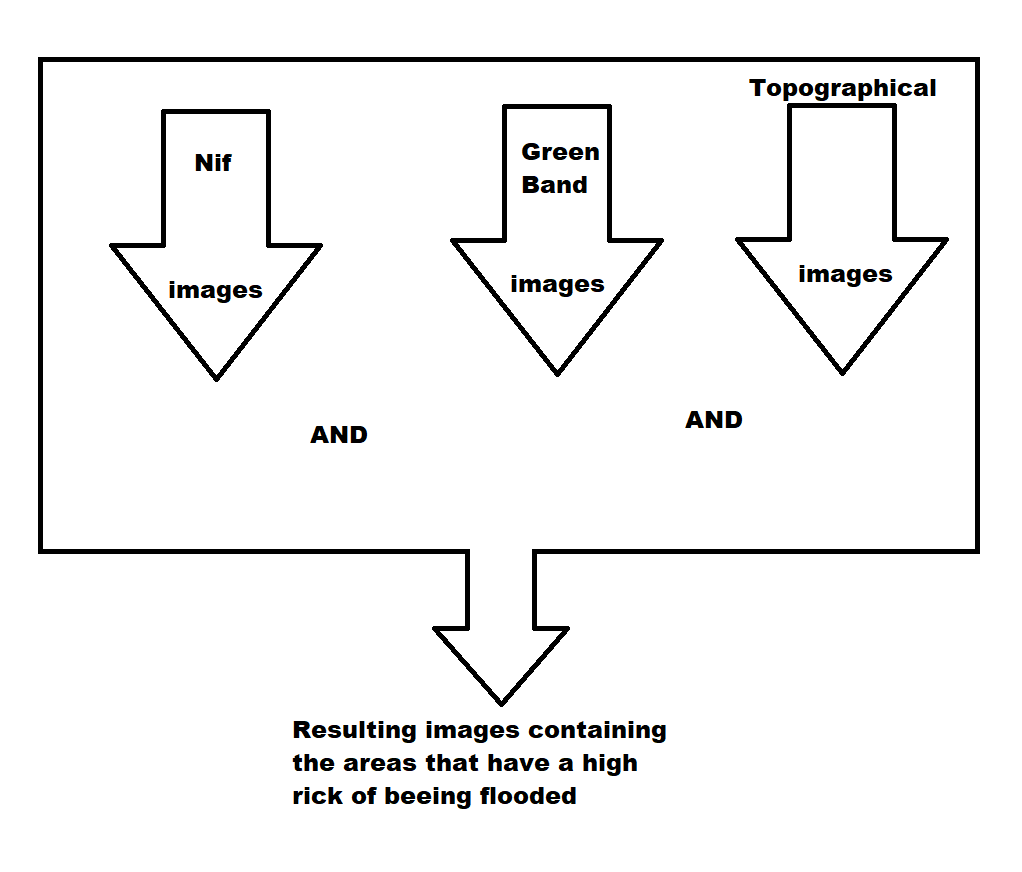
\includegraphics[scale=0.6]{application_outline.png} 
\end{center}

Combining those techniques with an easy to use and understand client interface we managed to create a system that can predict the land areas with a high potential of being flooded. The processing time and cost are reduced because the server part has to go through a set of images only twice, first time to detect the surface water and second time to fill the land area based on the topographic map, so the computations are reduced as low as possible. On the client side, there are big advantages because the set of resources (satellite images) are free and easy to access and the results are easy to understand, making this application ideal for a non trained person.
\par





\subsection{State of Art of Physically models in flood prediction}

\quad
For creating our physically prediction model we chose to use NDWI water extraction technique due its ease use and low processing time. McFeeters \cite{16} developed the normalized difference water index (NDWI) using the reflectance of the green (band 2) and near-infrared (band 4) bands of Landsat TM (Thematic Mapper). NDWI is one of the most widely used water indices for a variety of applications, including surface water mapping, land use/cover change analyses, and ecological research\cite{17-19} and also it shown great classification accuracy in areas that include shadow and dark surfaces.



\section{Thesis Structure}



\newpage{}


\chapter{Descrierea aplicatiei}

\section{Technologies used}

\subsection{Collecting and processing the resources}


\section{Programming languages and Frameworks} 

{\Large Programming language: Java\par}
\medskip


Java is popular high-level programming language that is object-oriented and it is designed to have as few implementation dependencies as possible. It was created in 1995 by Sun Microsystems and now it is owned by Oracle.
\par

This project was developed using Java 1.8 with two external libraries i.e.: Gdal and jai-imageio-core 1.4.0. Any version below 1.6 will now work as intended because of jai-imageio-core library. This library was used to process TIFF images from satellite.
\par

At first we intended to use Python as the heavy lifting programming language because of the more relaxed syntactic structure, but in the end we chose Java because of its parallel programming capabilities. Usually when we have to work with satellite images we should take into account the fact that the images can be really large, like 8161x7211 pixels in size covering over 589.000.000 $km^2$, and when we have to process more that one image of this kind the processing time becomes very important.
\par

Python will become much slower in this area because of the Global Interpreter Lock or GIL (a mutex, or a lock, that allows only one thread to hold the control of the Python interpreter). This means that only one thread can be in a state of execution at any point in time. The impact of the GIL isn’t visible to developers who execute single-threaded programs, but it can be a performance bottleneck in CPU-bound and multi-threaded code.
\par
\bigskip

In the following image we can take a look over the processing time between the Java's multi-threaded system and the single-threaded Python's system
\par

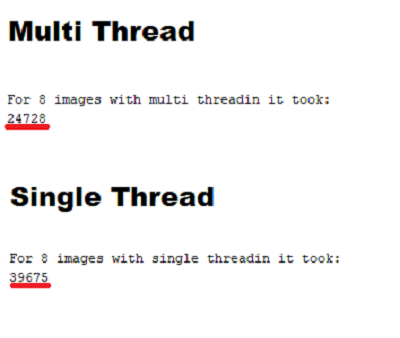
\includegraphics[scale=0.6]{multi_thread.png}
\par

{\Large Programming language: Python\par}
\medskip

Python is a interpreted, high-level, open source programming language that was made to have a  relaxed syntactic structure and to be more easy to read. It supports both functional and object oriented programming and its mainly targeted to a fast development and easy to maintain code.
\par

Python had played a major role in the project because of its relaxed syntactic structure and it was use to create the server part of the application, using Flask (flask is a microframework for python based applications).
\par 

After the server receives a set of satellite images from the user, a Java process is started by the server to solve the request. The java files are complied when the server is started for the first time and then for every request a java process is started. All this part was handled using the python's "subprocess" library
\par
\medskip

We will take a short look on how the python server compiles the java files and how a process is started, and we will discuss in more details in the next chapters.
\medskip

Here we can take a short look on how the java files are compiled
\par
\medskip
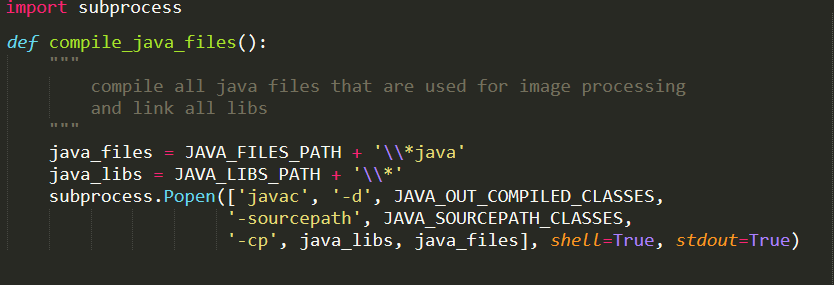
\includegraphics[scale=0.6]{python_call_java_1.png}
\bigskip

Here we can take a look on how a process is started
\par
\medskip
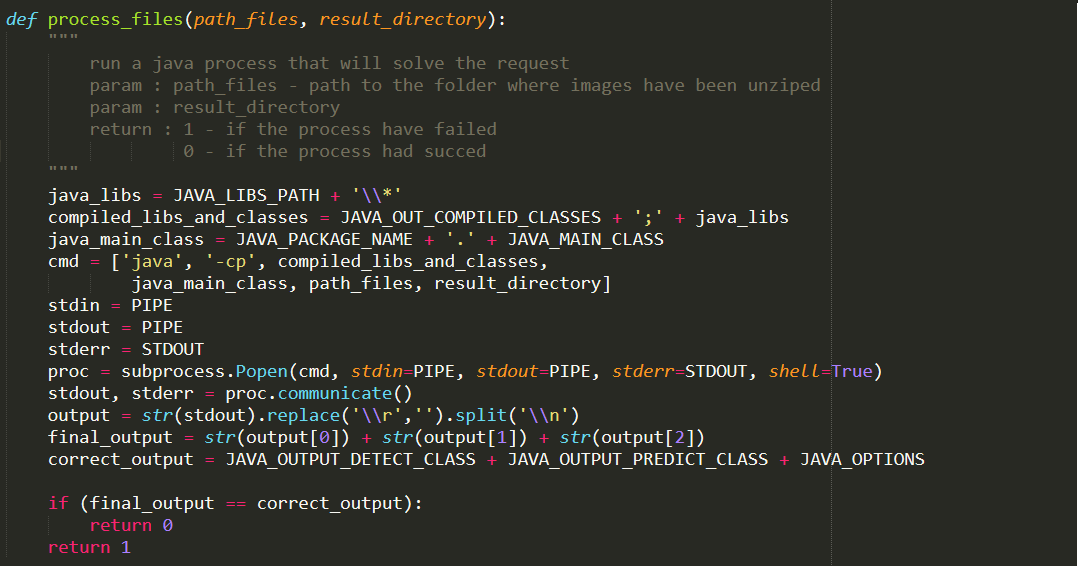
\includegraphics[scale=0.6]{python_call_java_2.png}



{\Large Features\par}

\begin{itemize}
  \item Coding assistance and analysis, with code completion, syntax and error highlighting, linter integration, and quick fixes
  \item Project and code navigation: specialized project views, file structure views and quick jumping between files, classes, methods and usages
  \item Python refactoring: including rename, extract method, introduce variable, introduce constant, pull up, push down and others
  \item Integrated Python debugger
  \item Integrated unit testing, with line-by-line code coverage
  \item Version control integration: unified user interface for Mercurial, Git, Subversion, Perforce and CVS with changelists and merge
\end{itemize}

\newpage{}

\section{Python Programming Language}

Python is an interpreted high-level programming language for general-purpose programming. Created by Guido van Rossum and first released in 1991, Python has a design philosophy that emphasizes code readability, notably using significant whitespace. It provides constructs that enable clear programming on both small and large scales. In July 2018, Van Rossum stepped down as the leader in the language community after 30 years.


Python features a dynamic type system and automatic memory management. It supports multiple programming paradigms, including object-oriented, imperative, functional and procedural, and has a large and comprehensive standard library.


Python interpreters are available for many operating systems. CPython, the reference implementation of Python, is open source software and has a community-based development model, as do nearly all of Python's other implementations. Python and CPython are managed by the non-profit Python Software Foundation. 


\newpage{}

\section{Gdal} 

	The Geospatial Data Abstraction Library (GDAL) is a computer software library for reading and writing raster and vector geospatial data formats, and is released under the permissive X/MIT style free software license by the Open Source Geospatial Foundation. As a library, it presents a single abstract data model to the calling application for all supported formats. It may also be built with a variety of useful command line interface utilities for data translation and processing. Projections and transformations are supported by the PROJ.4 library.

	The related OGR library (OGR Simple Features Library), which is part of the GDAL source tree, provides a similar ability for simple features vector graphics data.

	GDAL was developed mainly by Frank Warmerdam until the release of version 1.3.2, when maintenance was officially transferred to the GDAL/OGR Project Management Committee under the Open Source Geospatial Foundation.

	GDAL/OGR is considered a major free software project for its "extensive capabilities of data exchange" and also in the commercial GIS community due to its widespread use and comprehensive set of functionalities.

{\Large How to install Gdal on a Windows machine\par}

\begin{itemize}
  \item The user will need to install a version of Python
  \item The user will need to install the Miniconda packages Conda (recommended Conda - a more complex version of miniconda)
  \item The user will need to install the Gdal Api's using the following commands : conda install -c conda-forge gdal or conda install -c conda-forge/label/broken gdal
\end{itemize}



\newpage{}

\section{Qgis} 

QGIS (previously known as Quantum GIS) is a free and open-source cross-platform desktop geographic information system (GIS) application that supports viewing, editing, and analysis of geospatial data. 

{\Large Functionality \par}

	QGIS functions as geographic information system (GIS) software, allowing users to analyze and edit spatial information, in addition to composing and exporting graphical maps. QGIS supports both raster and vector layers; vector data is stored as either point, line, or polygon features. Multiple formats of raster images are supported, and the software can georeference images.

	QGIS supports shapefiles, coverages, personal geodatabases, dxf, MapInfo, PostGIS, and other formats. Web services, including Web Map Service and Web Feature Service, are also supported to allow use of data from external sources.

	QGIS integrates with other open-source GIS packages, including PostGIS, GRASS GIS, and MapServer. Plugins written in Python or C++ extend QGIS's capabilities. Plugins can geocode using the Google Geocoding API, perform geoprocessing functions similar to those of the standard tools found in ArcGIS, and interface with PostgreSQL/PostGIS, SpatiaLite and MySQL databases. 

{\Large How to install Qgis\par}

\begin{itemize}
  \item The user will need to download and install the Qgis Standalone Installer corresponding to the operating system 32/64
  \item Through the OSGeo4W shell's the user will be able to realise fast operations on the data from the satellites
\end{itemize}


\newpage{}


\chapter{The application}

\section{Qgis introduction} 


\section{Python GDAL introduction} 

\section{Functional description} 


\section{The user interface}


\section{Main use cases}


\section{Implementation details}

\newpage

\section{Application specification - user's point of view}

{\Large User's point of view\par}

This app should be able to deliver a marked zone on the land area(provided by the user), based on the probabilities of that zone to be floodable. (ex: red for high probability, green for none)\par 

The user will have to insert a set of images provided by sentinel 1,2 or 3, or a .tif representation of the area which he wants to test. The .tif set of images should include a infrared picture as well, because that is the way in which the water can be detected. The satellites usually use infrared scanners so this would not be a problem. The infrared images are useful because the water will absorb the infrared laser, so the areas covered with water are usually black. This is how the program will find the water areas, and will be able to detect the zones which have a higher chance of being flooded. Depending on the progress of the program, we will try to offer a GUI for the user in which he/she will be able to insert the coordinates of the area under the observation, and we will try to download the images based on their coordinated using a API for sentinel satellites.

\par 
The resulted image will give the user a sense of which areas are more likely of being flooded during a heavy rain period.

\newpage

\section{Application specification - programmer's point of view}

{\Large User's point of view and application skeleton\par}

This app should be able to deliver a marked zone on the land area(provided by the user), based on the probabilities of that zone to be floodable. (ex: red for high probability, green for none)\par 

The app will receive a set of .tif images, (provided by the user) from Landsat, sentinel 1,2 or 3, one image will be in infrared and the other one will be composed from the green wave channel.\par
 The way that we detect water is by combining the NIF(infrared) with green band resulting NDWI (Normalized Difference Water Index). NDWI  is a remote sensing based indicator sensitive to the change in the water content.NDWI  is computed  using  the  near  infrared  (NIR–MODIS  band  2)  and  the  short  wave infrared (Green band) reflectance’s.\par 
The formula will be applied as following for each pixel:

$$ NDWI/perpixel = \frac{Xgreen - Xnir}{Xgreen + Xnir}$$

If the resulted pixel has a value bigger that 0.45 we classify that specific pixel as a pixel that contains/is water (lake, river, ocean, etc), and all the pixels below that value as non-water pixels (land). We will color the water pixels in white and the other ones in black. \par 

Using this method we will obtain all the water content of a picture, and we can mark the areas which have a high risk of being flooded(the areas near the water). \par 

Later the user will be able to add a set of topographic images and determine the exact areas that will be flooded, by combining the results from NDWI water area detection with the topographic height of the map.




\newpage{}

\chapter{Conclusions}


\section{Performance Evaluation} 


\section{Future Development}

\newpage{}

\chapter{Bibliography} 

\section{References}

\begin{thebibliography}{widest entry}
\bibitem{Rover} Rover J., Ji L., Wylie B.K., Tieszen L.L. Establishing Water Body Areal Extent Trends in Interior Alaska from Multi-Temporal Landsat Data. Remote Sens. Lett. 2012;3:595–604. doi: 10.1080/01431161.2011.643507

\bibitem{Alsdorf} Alsdorf D.E., Rodríguez E., Lettenmaier D.P. Measuring Surface Water from Space. Rev. Geophys. 2007;45 doi: 10.1029/2006RG000197. [CrossRef] [Google Scholar]

\bibitem{Xie} Xie, K; Ozbay,K;Zhu, Y;Yang, H. Evacuation zone modeling under climate change: A data-driven method. J.Infrastruct. Syst. 2017,23,04017013

\bibitem{Pitt}Pitt, M.	Learning Lessons from the 2007 Floods; Cabinet Office: London, UK, 2008.

\bibitem{Lohani}Lohani, A.K.; Goel, N.; Bhatia, K. Improving real time flood forecasting using fuzzy inference system.J. Hydrol. 2014, 509, 25–41

\bibitem{Nayak}Nayak, P.; Sudheer, K.; Rangan, D.; Ramasastri, K. Short-term flood forecasting with a neurofuzzy model.Water Resour. Res. 2005, 41.

\bibitem{Fox}Fox, N.I.; Wikle, C.K. A bayesian quantitative precipitation nowcast scheme. Weather Forecast. 2005, 20, 264–275.

\bibitem{Merz}Merz, B.; Hall, J.; Disse, M.; Schumann, A. Fluvial flood risk management in a changing world. Nat. Hazards Earth Syst. Sci. 2010, 10, 509–527

\bibitem{Taherei}Taherei Ghazvinei, P.; Hassanpour Darvishi, H.; Mosavi, A.; Yusof, K.B.W.; Alizamir, M.; Shamshirband, S.; Chau, K.W. Sugarcane growth prediction based on meteorological parameters using extreme learning machine and artificial neural network. Eng. Appl. Comput. Fluid Mech. 2018, 12, 738–749

\bibitem{Kasiviswanathan}Kasiviswanathan, K.; He, J.; Sudheer, K.; Tay, J.-H. Potential application of wavelet neural network ensemble to forecast streamflow for flood management. J. Hydrol. 2016, 536, 161–173.

\bibitem{Ravansalar}Ravansalar, M.; Rajaee, T.; Kisi, O. Wavelet-linear genetic programming: A new approach for modeling monthly streamflow. J. Hydrol. 2017, 549, 461–475.

\bibitem{Mosavi}Mosavi, A.; Rabczuk, T. Learning and intelligent optimization for material design innovation. In Learning and Intelligent Optimization; Springer: Cham, Switzerland, 2017; pp. 358–363.

\bibitem{Dandagala}Dandagala, S.; Reddy, M.S.; Murthy, D.S.; Nagaraj, G. Artificial neural networks applications in groundwater hydrology—A review. Artif. Intell. Syst. Mach. Learn. 2017, 9, 182–187.

\bibitem{Deka}Deka, P.C. Support vector machine applications in the field of hydrology: A review. Appl. Soft Comput. 2014,
19, 372–386.

\bibitem{Fotovatikhah}Fotovatikhah, F.; Herrera, M.; Shamshirband, S.; Chau, K.-W.; Faizollahzadeh Ardabili, S.; Piran, M.J. Survey of computational intelligence as basis to big flood management: Challenges, research directions and future work. Eng. Appl. Comput. Fluid Mech. 2018, 12, 411–437. 

\bibitem{McFeeters}McFeeters, S.K. The use of the normalized difference water index (NDWI) in the delineation of open water features. Int. J. Remote Sens. 1996, 17, 1425–1432.

\bibitem{Duan}Duan, Z.; Bastiaanssen, W.G.M. Estimating water volume variations in lakes and reservoirs from four operational satellite altimetry databases and satellite imagery data. Remote Sens. Environ. 2013, 134, 403–416.

\bibitem{Poulin}Poulin, B.; Davranche, A.; Lefebvre, G. Ecological assessment of phragmites australis wetlands using multi-season spot-5 scenes. Remote Sens. Environ. 2010, 114, 1602–1609..

\bibitem{Hui}Hui, F.; Xu, B.; Huang, H.; Yu, Q.; Gong, P. Modelling spatial-temporal change of poyang lake using multitemporal landsat imagery. Int. J. Remote Sens. 2008, 29, 5767–5784.

\end{thebibliography}






% end appendix part

\end{document}
